\documentclass[a4paper 14pt]{extarticle}
\usepackage[utf8]{vietnam}
\usepackage{amsmath}
\usepackage{amsthm}
\usepackage{amsfonts}
\usepackage{amssymb}
\usepackage{float}
\usepackage[document]{ragged2e}
%for use of addmargin environment
\usepackage{scrextend}

\usepackage[margin = 1.5in]{geometry}
\usepackage{graphicx}
\graphicspath{{images/}}
\begin{document}
	\begin{titlepage}
\begin{center}
	\large{\textbf{ĐẠI HỌC QUỐC GIA THÀNH PHỐ HỒ CHÍ MINH}}\\
	\large{\textbf{TRƯỜNG ĐẠI HỌC KHOA HỌC TỰ NHIÊN}}\\
	\large{\textbf{KHOA CÔNG NGHỆ THÔNG TIN}}\\
	\vfill
	\begin{figure}[H]
		\centerline{
\includegraphics[scale = 0.5]{logo}}
	\end{figure}

	\Large{\textbf{Nhập môn phân tích độ phức tạp thuật toán}}\\
	\Large{\textbf{Báo cáo tìm hiểu P vs NP}}\\

\end{center}
	\vfill
\begin{flushright}
	
	\begin{tabular}{l l l}
		GVLT: &Thầy Trần Đan Thư\\
		&\\
		GVTH: &Thầy Nguyễn Đức Thân\\
		&Thầy Trương Toàn Thịnh\\
		&Thầy Nguyễn Vinh Tiệp\\
		&Thầy Nguyễn Sơn Hoàng Quốc\\
		&\\
		Nhóm:&13\\
		Sv: &Nguyễn Phan Mạnh Hùng & 1312727\\
		&Lục Kiến Nghiệp & 1312734\\
		&La Ngọc Thùy An & 1312716\\
		&Nguyễn Phước Đạt & 1312721\\
	\end{tabular}
\end{flushright}


\end{titlepage}

	\pagebreak

	\section{Tổng quan}
		\subsection{Phát biểu bài toán}
			Bài toán được phát biểu như sau: 
			\begin{quotation}
				Liệu tất cả các bài toán mà lời giải của nó có thể kiểm tra được trong thời gian đa thức có thể giải trong thời gian đa thức được hay không?
			\end{quotation}

		\subsection{Sơ lược về nguồn gốc bài toán}
		Bài toán được đề cập tới lần đầu trong một bức thư do Kurt Godel gửi tới John Von Neumann vào năm 1956. Trong đó Godel đặt vấn đề liệu các bài toán NP có thể giải trong thời gian tuyến tính hay bậc hai được không. Tuy vậy bài toán này được phát biểu một cách chính xác trong bài báo của Stephen Cook năm 1971, tên "The complexity of theorem proving procedures". Tuy bài toán bài toán này còn khá "non trẻ" nếu đặt lên bàn cân so với nhiều bài toán nổi tiếng khác, nhưng nó được xem là một trong những vấn đề quan trọng nhất lĩnh vực khoa học máy tính và toán học, và còn được xem như một cầu nối giữa hai lĩnh vực này. Chính bởi tính quan trọng của nó mà việc toán học Clay (Clay Mathematics Institute) đã lựa chọn nó là một trong 7 bài toán triệu đô.
		
		\subsection{Tầm quan trọng của bài toán}
		Để có thể hiểu rõ được tầm quan trọng của việc giải bài toán này ta sẽ thử nhìn từ 2 góc độ sau.\\
		Điều gì sẽ xảy ra nếu:
		\begin{itemize}
			\item P = NP
			\item P $\neq$ NP
		\end{itemize} 
			
			\subsubsection{P = NP}
				Nếu P = NP và, quan trọng hơn nữa, ta tìm được một cách giải hiệu quả cho một bài toán thuộc lớp NP-Complete. Khi đó, có thể nói, thế giới hoàn toàn thay đổi bởi khi ấy các ta có thể giải được các bài toán tối ưu một cách hiệu quả. Khi đó
				\begin{itemize}
					\item Ta có thể tạo ra các hệ thống lập lịch hoàn hảo để tiết kiệm tối đa nguồn lực, nâng cao hiệu suất, giảm thiểu lãng phí trong các bài toán di chuyển, xếp lịch làm việc.
					\item Ta có thể giải quyết nhiều vấn đề nan giải trong y học và chữa trị được nhiều bệnh nan y.
					\item Nâng cao khả năng học tập, học ít nhất nhưng đạt hiệu quả cao nhất.
					\item Và ta cũng có thể giải quyết hầu hết mọi bí ẩn mà khoa học chưa tìm ra đáp án.
				\end{itemize}  
				Tuy vậy, bên cạnh những lợi ích mang lại, thì nhân loại cũng phải đối mặt với nhiều vấn đề mà nó mang lại, đặc biệt là vấn đề an ninh. Bởi nhiều hệ thống an ninh được thiết lập dựa trên nền tảng của những bài toán khó, không chỉ là trong trường hợp xấu nhất mà còn phải đảm bảo các bài toán nền tảng này khó giải được trong các trường hợp trung bình. Nói rõ hơn, khi đó:
				\begin{itemize}
					\item Các hệ thống sử dụng mã công khai, public key, sẽ sụp đổ.
					\item Các hệ thống tín nhiệm (trusted third party, trusted servers) sẽ trở nên mất an toàn.
				\end{itemize}
			\subsubsection{P $\neq$ NP}
				Khi  P $\neq$ NP, chúng ta sẽ phải chấp nhận thế giới đầy những vấn đề không giải quyết được. Tuy vậy, con người cũng sẽ định hướng được cho việc giải quyết vấn đề, giả sử, nếu xác định được bài toán thuộc dạng NP. Khi đó, thay vì tập trung nguồn lực giải quyết trường hợp chung cho bài toán, ta sẽ tập trung giải quyết từng trường hợp đơn lẻ, cụ thể. Đó là việc vô cùng tích cực bởi trong thực tế, với lượng thông tin và các điều kiện thu thập được, thì bài toán dễ hơn rất nhiều, và cùng với việc năng lực tính toán của máy tính ngày càng cao thì ta cũng có thể giải được các bài toán khó với một quy mô khá lớn phù hợp với thực tế.\\
				
	\section{Định nghĩa}
		\subsection{Turing machine}
			Do các lớp bài toán được định nghĩa dựa trên nền tảng của Turing machine nên ta sẽ đề cập về khái niệm này đầu tiên.\\
			Có khá nhiều loại Turing machine được đề cập tới bao gồm:\\
			\begin{itemize}
				\item Deterministic Turing machine
				\item Non-deterministic Turing machine
				\item Probabilistic Turing machine
				\item Quantum Turing machine
				\item $\hdots$
			\end{itemize}
			Tuy vậy, trong giới hạn bài viết ta chỉ đề cập cụ thể tới 2 loại máy đầu tiên, do chúng có liên quan mật thiết đến các lớp bài toán phía sau.
			\subsubsection{Deterministic Turing machine}
				Một Turing machine được biểu diễn bởi 1 nhóm $M = \langle \Sigma, \Gamma, b, Q, \delta, q_0, F \rangle$\\
				Trong đó:\\
				\begin{tabular}{l p{4in}}
					$Q$& - tập hữu hạn, không rỗng gồm các trạng thái.\\
					$\Gamma$& - tập hữu hạn, không rỗng các kí tự trên đĩa(tape).\\
					$b \in \Gamma$& - kí tự trống (blank symbol), là kí tự duy nhất được xuất hiện vô số lần trên tape.\\
					$\Sigma \subseteq \Gamma \backslash \{b\}$& - tập hợp các kí tự input.\\
					$\delta: (Q \backslash F) \times \Gamma \to Q \times \Gamma \times \{L, R\} $& - là một hàm cục bộ (partial function) được gọi là một hàm chuyển (transition), L là dịch trái, R là dịch phải.\\
					$q_{0} \in Q$& - là trạng thái ban đầu.\\
					$F\subseteq Q$& - là tập trạng thái kết thúc hoặc chấp nhật (accepting states). Nội dung 1 tape được xem là chấp nhận bởi turing machine M khi và chỉ khi nó kết thúc với một trạng thái thuộc F. Thông thường $F = \{q_{accept}, q_{reject}\}$.\\
				\end{tabular}  
				Một cấu hình (configuration) của M được biểu diễn bởi 1 chuỗi $xqy$, trong đó $x, y \in \Gamma^{*}$, và được hiểu là M đang ở trạng thái $q$ với $xy$ trên đĩa (tape), và đầu đọc đang đọc kí tự đầu tiên của y.\\
				Một bước tính toán (computation - từ đây người viết sẽ sử dụng từ tiếng Anh gốc để bảo toàn nghĩa và làm cho bài viết xúc tích) được hiểu là một dãy các cấu hình $C_0, C_1, C_2, \hdots$, trong đó $C_0 = q_0w$, hoặc $C_0 = q_0b$ nếu $w$ là chuỗi rỗng. Bên cạnh đó $C_i \overset{M}{\to} C_{i+1}$. Khi đó, số bước tính toán bằng số cấu hình trừ 1.\\
				$\Sigma^*$ là tập các chuỗi tạo bởi các kí tự trong $\Sigma$\\
				Một ngôn ngữ (Language) ứng với tập kí tự $\Sigma$, gọi là $L$, và $L\subset \Sigma^*$.\\
				Một chuỗi $w \in L$ được gọi là chấp nhận bởi máy Turing (M), nếu ứng với chuỗi đó thì máy Turing sẽ dừng trong hữu hạn bước ở một trạng thái hợp lệ thuộc $F$.\\
				Gọi $L(M) = \{w, | w \in L,\text{M chấp nhận w} \}$.\\
				Gọi $t_M(w)$ là số bước máy Turing M chạy (số cấu hình trừ 1) ứng với input w.\\
				Khi đó $T_M(n) = Max\{t_M(w) | w \in \Sigma^n, n \in N\}$, n là độ dài của input. 
			\subsubsection{Non-deterministic Turing machine}
				Ta có thể định nghĩa Non-deterministic Turing machine (NTM) tương tự với Deterministic Turing machine (DTM). Điểm khác biệt duy nhất nằm ở $\delta$.\\
				Nếu ở DTM, thì $\delta$ là một hàm ánh xạ từ một cấu hình của máy Turing sang đúng 1 cấu hình khác hoặc không thể ánh xạ (theo định nghĩa của partial function). thì $\delta$ trong NTM thể hiện một quan hệ giữa 2 trạng thái.\\
				$\delta: (Q\backslash F \times \Gamma) \times (Q \times \Gamma \times \{L,R\})$\\
				Nói một cách đơn giản, từ một cấu hình hiện thời của NTM, ta có thể đi tới nhiều cấu hình khác, miễn chúng thỏa quan hệ $\delta$.\\
				Khi đó một chuỗi $w$ được gọi là chấp nhận bởi một NTM khi và chỉ khi tồn tại một đường đi (có thể có nhiều đường đi do tính chất của NTM) kết thúc với một trạng thái thuộc F.\\
				Nếu xem mỗi cấu hình trong dãy cấu hình ứng với một input sinh ra bởi Turing machine là một đỉnh của đồ thị, thì đồ thị ứng với DTM là một đường đi đơn, còn ứng với một NTM là một cây mà mỗi nhánh (hoặc đường đi) không nhất thiết là hữu hạn.\\
				Dựa vào đó ta có thể đưa ra nhận xét, nếu chuỗi w được chấp nhận bởi NTM, thì phải tồn tại một nhánh hữu hạn nút, mà nút lá mang trạng thái hợp lệ. Khi đó, ta định nghĩa $t_M(w)$ là độ dài của nhánh ngắn nhất chấp nhận w. Các định nghĩa khác là tương tự như với DTM.\\ 
		\subsection{Lớp bài toán P}
			Nói đơn giản lớp P bao gồm tất cả các bài toán mà tồn tại một thuật toán có thể đưa ra lời giải của nó trong thời gian đa thức.\\
			Trong đó P có nghĩa: Polynomial time.\\
			Ví dụ: tìm số lớn nhất trong dãy số nguyên, cộng 2 số nguyên lớn.
			
			Dựa trên định nghĩa về Deterministic Turing machine ở trên, ta có thể biểu diễn lại như sau.
			$P = \{L| L \in L(M), \forall w \in L, T_M(|w|) = w^k + h; k,h \in N\}$
			
			Ví dụ:\\
			\begin{description}
				\item[Bài toán kiểm tra số nguyên tố] Cho một số nguyên không âm, hãy kiểm tra đây có phải là số nguyên tố hay không. Trên thực tế, cho tới trước khi thuật toán AKS ra đời, thì các nhà khoa học vẫn chưa chứng minh được bài toán này thuộc lớp P. Tuy vậy, thuật toán AKS mang ý nghĩa về mặt lý thuyết nhiều hơn (chứng minh rằng bài toán kiểm tra số nguyên tố thuộc lớp P), nhưng trong thực tế thường ít được sử dụng bởi độ phức tạp lớn $\overset{~}{O(log^{12}(n))}$ (với giải thuật nguyên mẫu), và sau này được cải tiến xuống còn $\overset{~}{O(log^{7.5}(n))}$. Trong đó $g(x) = \overset{~}{O(f(x))}$ là viết tắt của $g(x) = O(f(x)log^k(f(x))$. Từ đó ta cũng nhận thấy rằng, các bài toán thuộc lớp P, trong thực tế chưa hẳn đã dễ "giải" hơn các bài toán thuộc lớp NP. Ở đây, ta xem việc "giải" bài toán, là đưa ra một lời giải chấp nhận được. Tuy vậy, vẫn có những bài toán thuộc lớp NP mà ta có thể đề ra các thuật toán có độ phức tạp trung bình rất nhỏ, thậm chí là hằng số.
			\end{description}
		\subsection{Lớp bài toán NP}
			Lớp NP bao gồm tất cả các bài toán quyết định mà lời giải của nó có thể kiểm tra được trong thơi gian đa thức.\\
			Trong đó NP có nghĩa: Non-deterministic Polynomial time.\\
			Ta có thể đưa ra định nghĩa tương tự như P, chỉ khác duy nhất mọi khái niệm ta dùng đều tương ứng với NTM thay vì DTM.\\
			Tuy nhiên, ta cũng có thể đưa ra một định nghĩa khác không dựa trên NTM như sau:\\
			Xét ngôn ngữ $L \subset \Sigma^{*}$.\\
			$L \subset NP$ khi và chỉ khi tồn tại quan hệ nhị phân $R \subset \Sigma^{*} \times \Sigma^{*}$, và:
			\begin{itemize}
				\item $\forall w \in \Sigma^{*}, x \in L \equiv \exists y \in \Sigma^{*}, |y| \in O(|w|^k) (w,y) \in R)$
				\item Ngôn ngữ $L_R = \{x\#y| (x,y) \in R\}$ trên bộ kí tự $\Sigma \cup \{\#\}$ được xác định bởi DTM trong thời gian đa thức.
			\end{itemize}
			Khi đó, y được gọi là certificate của x, và máy Turing xác định $L_R$ là verifier của L.\\
			\vspace{0.5cm}
			Để hiểu rõ hơn, ta sẽ phát biểu 1 bài toán thuộc lớp NP theo định nghĩa trên.\\
			Xét nhóm $Z_N$ và phần tử  $g \in Z_N$. \\
			$H = \{x | \exists y \in Z_N,~ g^y \equiv x (mod N)\}$\\
			Xét quan hệ:\\
			$R = \{x\#y \in (Z_N\times Z_N)| g^y \equiv x (mod N)\}$\\
			\textbf{Định nghĩa:} $log_g(x) = y$ trên nhóm $Z_N$, nếu  $\exists y \in Z_N,~ g^y \equiv x (mod N)$.\\
			\textbf{Đặt vấn đề:} Cho $Z_N,~g,~x$, hãy kiểm tra xem $log_g(x)$ có tồn tại hay không.\\
			\textbf{Nhận xét:} rõ ràng việc $log_g(x)$ tồn tại hay không tương đương với x có thuộc H hay không. Bên cạnh đó nếu xem y là certificate của x, và R là verifier của H, thì ta có chứng minh được $H \in NP$\\
			\vspace{0.5cm}
			
			Một số bài toán nổi tiếng thuộc lớp NP:\\ 
			\begin{description}
				\item[Bài toán tổng con] cho một dãy số, hay tìm một dãy con có tổng bằng 0. Ta có thể kiểm tra kết quả bài toán bằng một vòng lặp nhưng để tìm ra được kết quả thì vô cùng khó khăn ngoại trừ cách duyệt hết tất cả, $2^N$, tập con.
				\item[Bài toán Boolean Satisfiability] \label{EX: NP-C} cho một tập các biểu thức Boolean định nghĩa trên tập biến cho trước, liệu có tồn tại cách gán giá trị TRUE hay FALSE cho từng biến để tất cả các biểu thức đều mang giá trị TRUE hay không? Đây là một bài toán vô cùng quan trọng bởi nó được xem là bài toán thuộc lớp các bài toán khó nhất trong tất cả các bài toán NP. Điều này có nghĩa là nếu giải được bài toán này ta có thể giải được tất cả các bài trong lớp NP sử dụng thuật toán của nó. Hơn thế nữa, tất cả các bài toán trong lớp NP đều có thể rút gọn về bài toán này trong thời gian đa thức. Điều này mang ý nghĩa vô cùng lớn bởi nếu có thể tìm ra thuật toán trong thời gian đa thức cho bài toán này thì ta cũng có thể giải được tất cả các bài toán NP trong thời gian đa thức.
			\end{description}
		\subsection{Lớp bài toán NP-Hard}
			Lớp NP-Hard bao gồm tất cả các bài toán mà "có độ khó tối thiểu bằng các bài toán khó nhất trong lớp NP", nhưng không nhất thiết nằm trong lớp NP.\\
			Nói cách khác thì một bài toán A thuộc lớp NP-hard khi và chỉ khi với mỗi bài toán thuộc lớp NP, luôn tồn phép rút gọn trong thời gian đa thức về bài toán A.\\
			Phát biểu hình thức:
			\begin{addmargin}{0.5in}
				\begin{tabular}{l p{4in}}
				NPH& lớp các bài toán NP-hard.\\
				NP& lớp các bài toán NP.\\
				$\leq^{P}:$& phép rút gọn trong thời gian đa thức. (ta sẽ đề cập tới định nghĩa của phép tính này sau)\\
				Định nghĩa&$A \in NPH \Leftrightarrow \forall B \in NP,~ B \leq^{P} A$
				\end{tabular}
			\end{addmargin}
			Ví dụ:
			\begin{description}
				\item[Bài toán Knapsack]  Cho một túi sách với trọng lượng tối đa W. N đồ vật với trọng lượng $w_{i}$ và giá trị $v_{i}$. Hãy tìm tập con các đồ vật để bỏ vào túi sao cho tổng giá trị là lớn nhất có thể và tổng trọng lượng không vượt quá W.
			\end{description}
		\subsection{Lớp bài toán NP-Complete}
			Có nhiều cách để định nghĩa NP-Complete.\\
			Một trong số đó dựa trên định nghĩa về NP-Hard và NP.\\
			\begin{addmargin}{0.5in}
				\begin{tabular}{l l}
				NPC & lớp các bài toán NP-complete.\\
				Định nghĩa & $A \in NPC \Leftrightarrow A \in NPH \cap NP$\\
				hoặc & $A \in NPC \Leftrightarrow A \in NP\&~\forall B \in NP,~~B \leq^{P}A$\\
				\end{tabular}
			\end{addmargin}
			Ví dụ:
			\begin{description}
				\item[Bài toán Knapsack - phiên bản bài toán quyết đinh]  Cho một túi sách với trọng lượng tối đa W. N đồ vật với trọng lượng $w_{i}$ và giá trị $v_{i}$. Hỏi có thể bỏ các đồ vật vào túi sao cho tổng giá trị tối thiểu là V và trọng lượng không vượt quá W.
				\item[Bài toán Boolean Satisfiability] bài toán này phát biểu tương tự như ở ví dụ phần \ref{EX: NP-C}.
				\item[Bài toán Clique Cover] Xét một đồ thị tổng quát, hỏi có cách nào để phân các đỉnh của đồ thị trên thành k đồ thị con đầy đủ hay không.
			\end{description}
			Ví dụ về phép rút gọn một bài toán về bài toán thuộc lớp NP-Complete:\\
			Xét bài toán kiểm tra sắc số đồ thị (kiểm tra xem đồ thị có thể tô được bằng nhiều nhất k màu sao cho 2 đỉnh kề nhau tô màu khác nhau). Ta có thể biến đổi bài toán này về bài toán Clique Cover thông qua phép biến đổi trong thời gian đa thức như sau.\\
			\begin{enumerate}
				\item Xây dựng đồ thị bù của đồ thị cần kiểm tra sắc số. (Đồ thị G' gọi là bù của G nếu như $V_{G'} = V_{G}$ và 2 đỉnh u, v kề nhau trong G' khi và chỉ khi chúng không kề nhau trong G)
				\item Giải bài toán Clique Cover trên G'.
				\item Nếu câu trả lời là Yes, tức có thể phân G' thành k cliques thì ta cũng có thể tô đồ thị G bằng k màu, với các đỉnh trong cùng 1 clique của G' được tô cùng một màu. Do mỗi cặp đỉnh trong một clique của G' đôi một kề nhau, nên cũng có nghĩa là chúng đôi một không kề nhau trong G nên ta có thể tô cùng 1 màu.
			\end{enumerate}
	\section{Mối quan hệ giữa các lớp bài toán}
	\begin{figure}[H]
	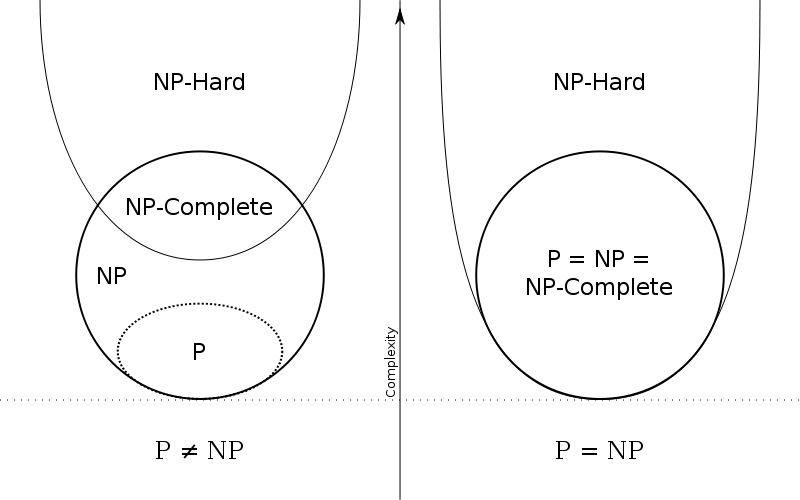
\includegraphics[scale = 0.4]{Venn.png}
	\end{figure}
	
	Dựa vào biểu trên, ta có nhận xét: nếu tồn tại một bài toán thuộc lớp NPC mà cũng thuộc lớp P thì khi đó NP = P. Điều này cũng dễ dàng chứng minh được dựa vào định nghĩa của lớp NPC. Đây cũng là một cách tiếp cận với bài toán \textbf{P vs NP}.
	
	\section{Tạm kết}
	Dù có giải được bài toán P vs NP hay không thì những ý nghĩa mà nó mang lại cho thế giới là vô cùng lớn. Bởi trong quá trình tìm hiểu, đề xuất, và xây dựng phương pháp để giải quyết bài toán này thì thế giới đã làm giàu thêm kho tàng kiến thức của mình đồng thời giúp cho chúng ta có cái nhìn sâu sắc hơn trong lĩnh vực phân tích độ phức tạp thuật toán.
\end{document}